\documentclass[a4paper]{article}
\usepackage[14pt]{extsizes}
\usepackage[utf8]{inputenc}
\usepackage[T2A]{fontenc}
\usepackage{amssymb,amsmath,mathtext}
\usepackage{indentfirst,amsfonts}
\usepackage[english, russian]{babel}
\usepackage{setspace}
\usepackage{graphicx}
\usepackage{pscyr}
\usepackage[left=30mm, top=20mm, right=10mm, bottom=20mm, nohead, footskip=10mm]{geometry} % настройки полей документа
\graphicspath{{graphs/}}
\onehalfspacing
\renewcommand{\rmdefault}{ftm} % Times New Roman
\renewcommand\refname{\centering СПИСОК ИСПОЛЬЗОВАННЫХ ИСТОЧНИКОВ}
\begin{document}
	%Титульный лист
	\begin{titlepage} % начало документа
	
	% НАЧАЛО ТИТУЛЬНОГО ЛИСТА
	\begin{center}
		\small{ФЕДЕРАЛЬНОЕ ГОСУДАРСТВЕННОЕ БЮДЖЕТНОЕ ОБРАЗОВАТЕЛЬНОЕ}\\ 
		УЧРЕЖДЕНИЕ ВЫСШЕГО ОБРАЗОВАНИЯ\\
		«МОСКОВСКИЙ ГОСУДАРСТВЕННЫЙ УНИВЕРСИТЕТ\\
		имени М.В.ЛОМОНОСОВА»\\
		\hfill \break
		%\normalsize{ФИЗИЧЕСКИЙ ФАКУЛЬТЕТ}\\
		ФИЗИЧЕСКИЙ ФАКУЛЬТЕТ \\
		\hfill \break
		КАФЕДРА МАТЕМАТИЧЕСКОГО МОДЕЛИРОВАНИЯ И ИНФОРМАТИКИ\\
		\hfill \break
		\hfill \break
		\hfill \break
		\hfill \break
		БАКАЛАВРСКАЯ РАБОТА\\
		\hfill \break
		\textbf{НЕЙРОСЕТЕВОЙ СИНТЕЗ ТЕКСТУР С ТРЕНДАМИ}\\
	\end{center}
	
	\hfill \break

	\begin{flushright}
		Выполнил студент \\
		435 группы:\\
		Будакян Я. С.\\
		\underline{\hspace{3cm}}\\
		\hfill \break
		Научный руководитель: \\
		к.т.н., доц. Грачев Е. А.\\
		\underline{\hspace{3cm}}
	\end{flushright}
	
	\begin{flushleft}
		Допущена к защите\\
		Зав. кафедрой \underline{\hspace{3cm}}\\
	\end{flushleft}
	\hfill \break
	\begin{center}
		Москва \\
		\hfill \break
		2017 
	\end{center}
	
	\thispagestyle{empty} % выключаем отображение номера для этой страницы
	
	% КОНЕЦ ТИТУЛЬНОГО ЛИСТА

\end{titlepage}  % КОНЕЦ ДОКУМЕНТА !
	%Учет титульного листа в нумерации
	\setcounter{page}{2}
	\tableofcontents
	\addcontentsline{toc}{section}{ВВЕДЕНИЕ}
	% ВВЕДЕНИЕ
	\clearpage
\section*{\hfil ВВЕДЕНИЕ \hfil}
	В современной добыче полезных ископаемых активно применяются средства математического моделирования для симуляции процессов, происходящих в пласте. Однако, на данный момент полноценное моделирование не представляется возможным, поэтому используются различные приближенные методы. Для правильной симуляции процессов, происходящих в недрах, необходимо смоделировать саму среду, в которой эти процессы протекают. Обычно, данные о структуре среды доступны только в некотором количестве точек (скважин), в которых непосредственно идет добыча. Предлагается попытаться использовать методы машинного обучения для синтеза модели среды, похожей на природную. В рамках решения этой проблемы возникает задача синтеза текстур с трендами, например, для учета каких-либо пространственных корреляций. 
	
	Под текстурой с трендом в данном случае понимается изображение, в котором есть изменение некоторой статистической характеристики вдоль одного из направлений. Такими характеристиками, например, могут быть изменение интенсивности появления частиц среды или пористости среды.
	
	Базовым подходом в задаче синтеза текстур на данный момент является использование искусственных нейросетей. Однако, известные работы в области синтеза текстур с помощью искусственных нейросетей \cite{texture-synthesis-using-CNN, texture-networks} показывают, что у нейросетевых моделей есть проблемы с воспроизведением формы объектов, а также различных пространственно скоррелированных структур. Соответственно, целью данной работы ставится поиск нейросетевой архитектуры, способной улавливать и воспроизводить протяженные корреляции.
	
	Для упрощения задачи, будем в дальнейшем рассматривать множество изображений с трендами, удовлетворяющее следующим ограничениям:
	
	\begin{itemize}
		\item Это монохромные изображения 256 x 256 пикселей
		\item Изменяющимся свойством является интенсивность появления частиц $\lambda$
		\item Тренд является линейным и направлен вдоль оси изображения $z_1$: 
		$ \lambda = \lambda_{init} + k z_1 $
		\item По оси $z_2$ остается равномерное распределение частиц
	\end{itemize}
	
	Каждый такой тренд фиксируется значениями $\lambda_{init}$ и $\lambda_{final}$. Следовательно, 
	$$k = \frac{\lambda_{final} - \lambda_{init}}{256}$$
	Пример такого изображения с трендом интенсивности приведен на (Рис. \ref{1-trend-example}):
	
	\begin{figure}[h]
		\centering{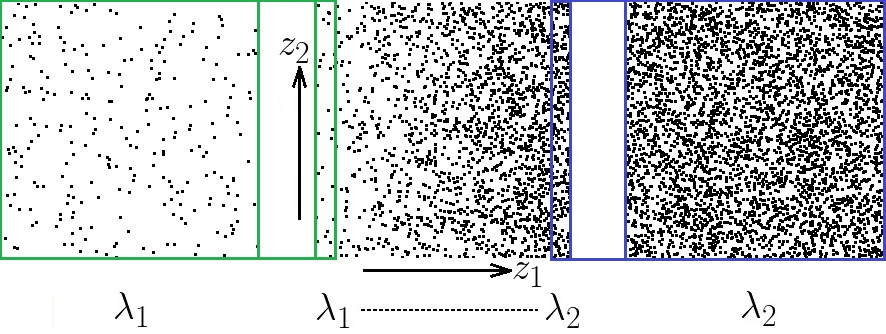
\includegraphics[width=\linewidth]{1-introduction/trend-example}}
		\caption{Пример изображения с трендом, фиксируемого двумя изображениями}
		\label{1-trend-example}
	\end{figure}
	
	Математически сформулировать постановку описанной задачи можно с помощью так называемой вероятностной постановки задачи обучения \cite{Voron-ML, GAN-original}.
	
	Рассмотрим многомерное пространство $X$, содержащее множество всех изображений $x$: $X = \{x\}$. Пусть у нас есть обучающая выборка из изображений, содержащих в себе рассматриваемое множество трендов $D = \{x_i\}$. Тогда считается, что  обучающая выборка изображений с трендами $D$ задает в этом пространстве вероятностное распределение $P_X : X \longrightarrow [0,1]$, устроенное таким образом, что точки, соответствующие изображениям из выборки, имеют высокую вероятность, а остальные - низкую. Таким образом, с математической точки зрения задача синтеза текстуры с трендом сводится к синтезу случайного изображения $x'$, принадлежащего распределению, близкому к задаваемому обучающей выборкой:
	$$ P_{X'} \approx P_X, \quad x' \sim X'$$
	
	``Классический'' статистический подход к решению подобного рода задач заключается в введении в рассмотрение параметризированного семейства распределений вероятности и его подстройке к имеющимся данным:
	
	\begin{itemize}
		\item Вводится параметризированное семейство распределений вероятности $P_{\theta}(x)$
		\item Параметры $\theta$ находятся из обучающей выборки:
		$$ \mathcal{L}_{\theta}(D) = \prod_{x \in D} P_{\theta}(x) $$
		$$ \theta^{*} = \underset{\theta}{\arg\max} \mathcal{L}_{\theta}(D)$$
		\item Генерируется объект (изображение) из распределения $ P_{\theta^{*}}$
	\end{itemize}
	
	Этот подход приводит к проблемам:
	
	\begin{itemize}
		\item Пространство параметров $\theta$ может быть огромной размерности
		\item Известной параметрической модели распределения может вообще не существовать
	\end{itemize}
	
	Простой пример объекта со сложным пространством параметров - человеческое лицо. Задачу генерации изображения реалистичного человеческого лица долгое время не могли решить с удовлетворительным качеством. Однако последние достижения в области искусственных нейронных сетей привели к существенному улучшению качества генеративных моделей самого разнообразного типа. В частности, впечатляющие результаты были достигнуты с помощью генеративных состязательных сетей (GAN) \cite{cGAN, cGAN-face, EBGAN, BEGAN}, что мотивирует попытку применения нейросетей этой архитектуры в поставленной задаче.
	
	\subsection*{Постановка задачи}
	
	Таким образом, для достижения обозначенной во введении цели, поставить задачу работы можно так:
	
	\begin{itemize}
		\item Разработать модифицированные для синтеза описанного множества текстур с трендами архитектуры GAN
		\item Провести вычислительные эксперименты, связанные с обучением нейросетей (то есть, с решением задач многопараметрической оптимизации)
		\item Синтезировать с помощью обученных нейросетей новые текстуры и верифицировать их
	\end{itemize}
	% Постановка задачи
	\section{Постановка задачи}
	Математически сформулировать поставленную задачу можно с помощью так называемой вероятностной постановки задачи обучения \cite{Voron-ML, GAN}.
	Рассмотрим многомерное пространство $X$, содержащее множество всех изображений $x$: $X = \{x\}$. Тогда обучающая выборка изображений с трендами $D = \{x_i\}$ задает в этом пространстве вероятностное распределение $P_X : X \longrightarrow [0,1]$, устроенное таким образом, что точки, соответствующие изображениям из выборки, имеют высокую вероятность, а остальные - низкую. Тогда с математической точки зрения задача синтеза текстуры с трендом сводится к синтезу случайного изображения $x'$, принадлежащего распределению, близкому к задаваемому обучающей выборкой:
	$$ P_{X'} \approx P_X, \quad x' \sim X'$$
	
	"Классический" статистический подход к решению подобного рода задач заключается в введении в рассмотрение параметризированного семейства распределений вероятности и его подстройке на имеющихся данных:
	\begin{itemize}
		\item Вводится параметризированное семейство распределений вероятности $P_{\theta}(x)$
		\item Параметры $\theta$ находятся из обучающей выборки:
		$$ \mathcal{L}_{\theta}(D) = \prod_{x \in D} P_{\theta}(x) $$
		$$ \theta^{*} = \underset{\theta}{\arg\max} \mathcal{L}_{\theta}(D)$$
		\item Генерируется объект(изображение) из распределения $ P_{\theta^{*}}$
	\end{itemize}
	Этот подход приводит к проблемам:
	\begin{itemize}
		\item Пространство параметров $\theta$ может быть огромной размерности
		\item Известной параметрической модели распределения может вообще не существовать
	\end{itemize}
	Простой пример объекта со сложным пространством параметров - человеческое лицо. Задачу генерации изображения реалистичного человеческого лица долгое время не могли решить с удовлетворительным качеством. Однако последние достижения в области искуственных нейронных сетей привели к существенному повышению качества генеративных моделей самого разнообразного типа. Собственно, наличие впечатляющих работ последних лет в этой области \textbf{*тут цитаты*} и мотивирует попытаться применить современные нейросетевые подходы в поставленной задаче.
	% Нейронные сети
	\clearpage
\section{Нейронные сети}
	В общем смысле, искусственная нейронная сеть - это математическая модель, построенная по принципу организации и функционирования биологических нейронных сетей. Она представляет из себя систему соединенных простых блоков - искусственных нейронов, каждый из которых имеет входы и выходы для взаимодействия с другими нейронами. Главное преимущество нейронных сетей перед традиционными алгоритмами в том, что они обучаются на некотором наборе данных, а не программируются в классическом смысле этого понятия. Процесс обучения заключается в нахождении оптимальных весовых коэффициентов между нейронами. С математической точки зрения, процесс обучения - это задача многопараметрической нелинейной оптимизации.
	\subsection{Математическая модель нейрона}
		Одиночный нейрон обычно представляет собой взвешенный сумматор с нелинейной функцией активации на выходе:
		$$x_{out} = \phi(\vec{w} \cdotp \vec{x_{in}}),$$
		где $\vec{w}$ - вектор весовых коэффициентов связей, $\vec{x_{in}}$ - входной вектор, $\phi$ - нелинейная функция активации (Рис. \ref{3-artificial-neuron-model}).
		
		\begin{figure}[h]
			\centering{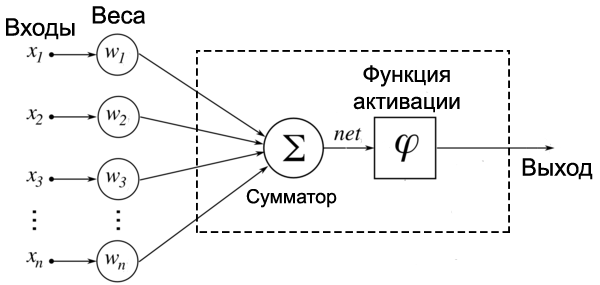
\includegraphics[width=0.9\linewidth]{3-ann/artificial-neuron-model}}
			\caption{Математическая модель нейрона}
			\label{3-artificial-neuron-model}
		\end{figure}
		
		Функция активации может выбираться разной в зависимости от задачи. Наиболее часто используемые функции:
		
		\begin{itemize}
			\item Сигмоида (логистическая функция)
					$$\sigma(x) = \frac{1}{1 + e^{-x}}$$
			\item Гиперболический тангенс
			\item ReLU
					$$ReLU(x) = \max(0, x)$$
			\item softmax
					$$\sigma(\vec{x})_j = \frac{e^{x_j}}{\sum_{k=1}^{N} e^{z_k}}$$
		\end{itemize}
		Множество таких нейронов объединяется в сеть и обучается каким-либо методом оптимизации.
	\subsection{Метод обратного распространения ошибки}
		Метод обратного распространения ошибки (backpropagation) - самый широко используемый и успешный алгоритм обучения глубоких (многослойных) нейронных сетей. Суть этого метода заключается в распространении сигналов ошибки от выходов сети к ее входам в обратном к распространению сигнала в сети направлении. Это позволяет вычислить производные ошибки по весам сети, которые потом можно использовать в любом градиентном алгоритме оптимизации (например, в стохастическом градиентном спуске).
		
		Обозначим множество входов сети как $\{x_1, \ldots, x_n\}$, множество выходов - $O$, $w_{ij}$ - вес, присвоенный ребру, соединяющему $i$-й и $j$-й узлы, $y_k$ - известные (правильные) ответы, $o_i$ - выход $i$-го узла. Введем функцию ошибки (например, сумма квадратов расстояний):
		$$ L(\vec{x}, W) = \frac{1}{2} \sum_{k \in O} (y_k - o_k)^2, $$
		где $W = \{w_{ij}\}$ - матрица весовых коэффициентов
		
		Рассмотрим сначала нейроны последнего слоя. Весовой коэффициент $w_{ij}$ влияет на выход сети как часть суммы $S_j = \sum_i w_{ij} x_i$. Соответственно,
		$$ \frac{\partial L}{\partial w_{ij}} = \frac{\partial L}{\partial S_j} \frac{\partial S_j}{\partial w_{ij}} = x_i \frac{\partial L}{\partial S_j} $$
		
		Аналогично, $S_j$ влияет на общую ошибку только в рамках выхода $j$-го узла $o_j$, поэтому
		$$ \frac{\partial L}{\partial S_j} = \frac{\partial L}{\partial o_j} \frac{\partial o_j}{\partial S_j}  = (\frac{\partial}{\partial o_j} \frac{1}{2} \sum_{k \in Out} (y_k - o_k)^2)(\frac{\partial \phi(S)}{\partial S} \bigg|_{S = S_j})$$
		Если узел $j$ не находится на последнем слое, то у него есть набор связей с нейронами следующего слоя. Обозначим их множество как $K_j$. Тогда
		$$ \frac{\partial L}{\partial S_j} = \sum_{k \in K_j} \frac{\partial L}{\partial S_k} \frac{\partial S_k}{\partial S_j} $$
		$$ \frac{\partial S_k}{\partial S_j} = \frac{\partial S_k}{\partial o_j} \frac{\partial o_j}{\partial S_j} = w_{jk}\frac{\partial o_j}{\partial S_j} $$
		$ \frac{\partial L}{\partial S_k}$ - аналогичная поправка, но для нейрона следующего слоя. В итоге, получены выражения для производных ошибки по весам для нейронов выходного слоя, а аналогичные производные для нейронов внутренних слоев выражены через нейроны следующих слоев. Это и есть процесс обратного распространения ошибки - градиенты ошибки по весам вычисляются последовательно, начиная с выходного слоя и заканчивая первым.
	\subsection{Сверточные нейронные сети}
		Сверточные нейронные сети (CNN - convolutional neural networks)- это специальная архитектура нейронной сети, нацеленная на эффективное распознавание изображений, впервые предложенная Яном Лекуном \cite{CNN-original}. Структура такой сети имеет некоторое сходство со строением зрительной коры головного мозга. Свое название CNN получили из-за наличия сверточных слоев, в которых каждый фрагмент изображения умножается на ядро свертки, полученный результат суммируется и записывается в аналогичную позицию выходного изображения. Одно отдельное ядро свертки обычно интерпретируют как кодирование какого-либо признака изображения. При этом сами ядра выучиваются сетью самостоятельно, а не закладываются человеком. В CNN чередуются сверточные слои и субдискретезирующие слои, таким образом более глубокие сверточные слои могут выделять абстрактные детали изображения, вплоть до общих понятий, таких как "кошка", "собака", и т.п. На данный момент CNN считаются базовым нейросетевым подходом при работе с изображениями.
	\subsection{Генеративные состязательные сети}
		Архитектура нейронной сети, получившая название генеративной состязательной сети (generative adversarial network - GAN), впервые была описана в 2014 году \cite{GAN-original}. За последнее время сети такого типа добились больших успехов в задачах синтеза объектов из сложных распределений. Этим объясняется мотивация попытки применения данной архитектуры для решения поставленной задачи.
		\subsubsection{Общая структура}
			Переформулируем изначальную задачу нахождения такой процеруды синтеза $X'$, что $ P_{X'} \approx P_X$:
			$$ \rho(P_{X'}, P_X) \longrightarrow \underset{P_{X'}}{\min} $$
			Введем параметризированную процедуру генерации:
			$$ X' = g_{\theta}(\cdot) $$
			Получаем:
			$$ \rho(P_{X'}, P_X) \longrightarrow \underset{P_{X'}}{\min} $$
			$$ \rho(g_{\theta}(\cdot), P_X) \longrightarrow \underset{g_{\theta}(\cdot)}{\min} $$
			$$ \rho(g_{\theta}(\cdot), P_X) \longrightarrow \underset{\theta}{\min} $$
			Возникает вопрос: что использовать в качестве метрики похожести двух распределений $\rho$, где одно из распределений задано обучающей выборкой.
			В качестве такой метрики можно использовать функцию потерь обученного классификатора, потому что естественно предположить, что чем чаще ошибается обученный классификатор, тем больше одно распределение похоже на другое. Тогда задача примет вид:
			$$ \rho(P_{X'}, P_X) \longrightarrow \min \Leftrightarrow L \longrightarrow \max, $$
			где $L$ - функция потерь обученного классификатора.
			Соответственно, можно ввести две нейросети:
	
			\begin{itemize}
				\item $d_{\zeta}(x)$ - классификатор для измерения расстояния, ``дискриминатор''
				\item $g_{\theta}(x)$ - сеть, трансформирующая шум в $X'$, ``генератор''
			\end{itemize}
	
			Суть использования двух сетей состоит в том, что они обучаются совместно, конкурируя друг с другом: генератор пытается имитировать целевое распределение, а дискриминатор пытается классифицировать поступающие от генератора и из обучающей выборки изображения на 2 класса: реальные (из изначального распределения $P_X$) и ложные (из $P_{X'}$, т.е. произведенные генератором).
			Для дальнейшего рассмотрения введем функцию потерь дискриминатора(например, logloss):
			$$ l_1 = l(d_{\zeta}(x), 1) \text{ - ошибка 1 рода} $$
			$$ l_2 = l(d_{\zeta}(x'), 0) \text{ - ошибка 2 рода}$$
			$$ L(X, X') = \frac{1}{2} \mathbb{E}_{X} l_1 + \frac{1}{2} \mathbb{E}_{X'} l_2 = -\frac{1}{2} (\mathbb{E}_{X} \log d_{\zeta}(x) + \mathbb{E}_{X'} \log (1 - d_{\zeta}(x'))) = $$
			$$ =  -\frac{1}{2} (\mathbb{E}_{X} \log d_{\zeta}(x) + \mathbb{E}_{V} \log (1 - d_{\zeta}(g_{\theta}(v)))) = L(\zeta, \theta) .$$
			Функция потерь обученного классификатора:
			$$ L^*(\theta) = \underset{\zeta}{\min} L(\zeta, \theta) $$
			Соответственно,
			$$ \underset{\zeta}{\min} L(\zeta, \theta) \longrightarrow \underset{\theta}{\max} $$
			$$ \theta^* = \underset{\theta}{\arg\max} \left[ \underset{\zeta}{\min} L(\zeta, \theta) \right] $$
			Определим оптимальный дискриминатор:
			$$ d^*_{\theta} = d_{\zeta^*(\theta)} $$
			$$ \zeta^*(\theta) =  \underset{\zeta}{\arg\min} L(\zeta, \theta)$$
		\subsubsection{Обучение GAN}
			Итак, задача обучения GAN свелась к нахождению
			$$ \theta^* = \underset{\theta}{\arg\max} \left[ \underset{\zeta}{\min} L(\zeta, \theta) \right] $$
			В итоге, процесс обучения принимает следующий вид:
	
			\begin{itemize}
				\item Обучаем дискриминатор при фиксированном генераторе
				\item Обучаем генератор при фиксированном дискриминаторе
				\item Повторяем до сходимости параметров обеих моделей
			\end{itemize}
			Описанный процесс схематично изображен на (Рис. \ref{5-gan-training}).
	
			\begin{figure}[h!]
				\centering{\includegraphics[width=0.4\linewidth]{5-GAN/gan-training}}
				\caption{Схематическое изображение процесса обучения GAN.}
				\label{5-gan-training}
			\end{figure}
	
		\subsubsection{Модификация ``pix2pix GAN''}
			Для решения задачи была опробована модификация обычной структуры GAN под названием ``pix2pix GAN'' \cite{pix2pix, p2p-vessnet}. Ее отличие от схемы GAN, введенной выше, состоит в том, что вместо шума на вход генератору приходят другие изображения, на которых он основывается при синтезе. Схематически ее устройство изображено на (Рис. \ref{5-p2p}).
	
			\begin{figure}[h!]
				\centering{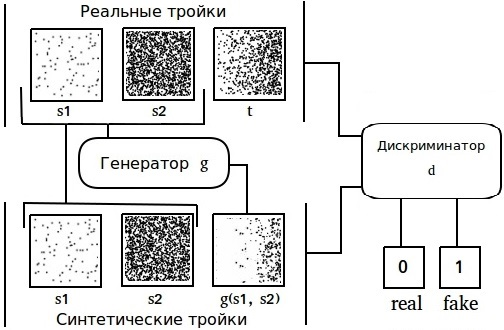
\includegraphics[width=0.75\linewidth]{5-GAN/p2p}}
				\caption{Схематическое устройство сети pix2pix GAN.}
				\label{5-p2p}
			\end{figure}
	
			Для pix2pix сети общий функционал потерь выглядит следующим образом: $$ L(G, D) = L_{adv}(G, D) + \eta L1$$
			$$L1 = \mathbb{E}_{p_{data}(s_1, s_2, r)} (\parallel r - G(s_1, s_2) \parallel_1)$$
			$$ L_{adv}(G, D) = \mathbb{E}_{p_{data}(s_1, s_2, r)}\log D(s_1, s_2, r) +  \mathbb{E}_{p_{data}(s_1, s_2)} \log (1 - D(s_1, s_2, G(s_1, s_2)))$$
			где G, D - генератор и дискриминатор, $(s_1, s_2, r)$ - тройка изображений (интенсивность слева, справа и реальное изображение с трендом),  $\mathbb{E}_{p_{data}(s_1, s_2, r)}$ - мат. ожидание логарифмического правдоподобия того, что тройка изображений $(s_1, s_2, r)$ принадлежит вероятностному распределению реальных троек $p_{data}(s_1, s_2, r)$, а $p_{data}(s_1, s_2)$ соответствует распределению реальных изображений $s_1, s_2$.
	
			В качестве генератора в \cite{pix2pix, p2p-vessnet} использовалась сеть ``U-Net'' \cite{unet}. Основное отличие сети ``U-Net'' от обычной сети архитектуры ``encoder-decoder'' заключается в наличии прямых связей между сверточными и разверточными слоями. Использование такого типа генератора позволяло увеличить качество синтезируемых изображений. Схемы сетей типа ``U-Net'' и ``Encoder-decoder'' приведены на (Рис. \ref{5-unet-sheme}).
			
			\begin{figure}[h!]
				\centering{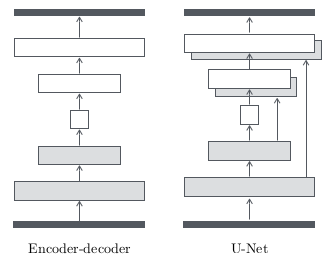
\includegraphics[width=0.65\linewidth]{5-GAN/unet-encoder}}
				\caption{Схематическое изображение нейросети-генератора.}
				\label{5-unet-sheme}.
			\end{figure}
	% Сверточная арифметика, сверточные сети
	\section{Сверточные нейронные сети}
	\subsection{Сверточная арифметика}
	\subsection{Сверточные слои}
	% GAN
	\section{Генеративные состязательные сети}
	Архитектура нейронной сети, получившая название генеративной состязательной сети (generative adversarial network - GAN), впервые была описана в 2014 году \cite{GAN}. В последние 2 года сети такого типа добились больших успехов в задачах синтеза объектов из сложных распределений (например, лиц) \cite{cGAN-face}, переноса стиля \cite{algorithm-of-articsic-style} и подобных. Этим объясняется мотивация попытки применения данной архитектуры для решения поставленной задачи.
	\subsection{Общая структура}
		Переформулируем изначальную задачу нахождения такой процеруды генерирования $X'$, чтобы $ P_{X'} \approx P_X$:
		$$ \rho(P_{X'}, P_X) \longrightarrow \underset{P_{X'}}{\min} $$
		Введем параметризированную процедуру генерации:
		$$ X' = g_{\theta}(\cdot) $$
		Переформулируем:
		$$ \rho(P_{X'}, P_X) \longrightarrow \underset{P_{X'}}{\min} $$
		$$ \rho(g_{\theta}(\cdot), P_X) \longrightarrow \underset{g_{\theta}(\cdot)}{\min} $$
		$$ \rho(g_{\theta}(V), P_X) \longrightarrow \underset{\theta}{\min} $$
		Возникает вопрос: что использовать в качестве метрики похожести двух распределений $\rho$, где одно из распределений задано обучающей выборкой.
		В качестве такой метрики можно использовать функцию потерь обученного классификатора, потому что естественно предположить, что чем чаще ошибается обученный классификатор, тем больше одно распределение похоже на другое. Тогда задача примет вид:
		$$ \rho(P_{X'}, P_X) \longrightarrow \min \Leftrightarrow L \longrightarrow \max, $$
		где $L$ - функция потерь обученного классификатора.
		Соответственно, можно ввести две нейросети:
		\begin{itemize}
			\item $d_{\zeta}(x)$ - классификатор для измерения расстояния, \textbf{'дискриминатор'}
			\item $g_{\theta}(x)$ - сеть, трансформирующая шум в $X'$, \textbf{'генератор'}
		\end{itemize}
		
		Суть использования двух сетей состоит в том, что они обучаются совместно, конкурируя друг с другом: генератор пытается имитировать целевое распределение, а дискриминатор пытается классифицировать поступающие от генератора и из обучающей выборки изображения на 2 класса: реальные (из изначального распределения $P_X$) и ложные (из $P_{X'}$, т.е. произведенные генератором).
		Для дальнейшего рассмотрения введем функцию потерь дискриминатора(например, logloss):
		$$ l_1 = l(d_{\zeta}(x), 1) \text{ - ошибка 1 рода} $$
		$$ l_2 = l(d_{\zeta}(x'), 0) \text{ - ошибка 2 рода}$$
		$$ L(X, X') = \frac{1}{2} \mathbb{E}_{X} l_1 + \frac{1}{2} \mathbb{E}_{X'} l_2 = -\frac{1}{2} (\mathbb{E}_{X} \log d_{\zeta}(x) + \mathbb{E}_{X'} \log (1 - d_{\zeta}(x'))) = $$
		$$ =  -\frac{1}{2} (\mathbb{E}_{X} \log d_{\zeta}(x) + \mathbb{E}_{V} \log (1 - d_{\zeta}(g_{\theta}(v)))) = L(\zeta, \theta) .$$
		Функция потерь обученного классификатора:
		$$ L^*(\theta) = \underset{\zeta}{\min} L(\zeta, \theta) $$
		Соответственно,
		$$ \underset{\zeta}{\min} L(\zeta, \theta) \longrightarrow \underset{\theta}{\max} $$
		$$ \theta^* = \underset{\theta}{\arg\max} \left[ \underset{\zeta}{\min} L(\zeta, \theta) \right] $$
		Определим оптимальный дискриминатор:
		$$ d^*_{\theta} = d_{\zeta^*(\theta)} $$
		$$ \zeta^*(\theta) =  \underset{\zeta}{\arg\min} L(\zeta, \theta)$$
	\subsection{Обучение GAN}
		Итак, задача обучения GAN свелась к нахождению
		$$ \theta^* = \underset{\theta}{\arg\max} \left[ \underset{\zeta}{\min} L(\zeta, \theta) \right] $$
		Решить ее можно, например, методом стохастического градиентного спуска:
		$$ \Delta \theta \sim \nabla L(\zeta^*(\theta), \theta)$$
		Для малых изменений $\Delta \theta$:
		$$ \nabla L(\zeta^*(\theta), \theta) \approx \nabla L(\zeta^*(\theta), \theta + \Delta \theta) $$
		В итоге, процесс обучения принимает следующий вид:
		\begin{itemize}
			\item Обучаем дискриминатор при фиксированном генераторе
			\item Обучаем генератор при фиксированном дискриминаторе
			\item Повторяем до сходимости параметров обеих моделей
		\end{itemize}
		\begin{figure}
			\centering{\includegraphics[width=0.4\linewidth]{gan-training}}
			\caption{Схематическое изображение процесса обучения GAN.}
			\label{gan-training}
		\end{figure}
	\subsection{Различные модификации}
		\subsubsection{pix2pix GAN}
			Для решения задачи было попробовано применить модификацию GAN-сети под названием "pix2pix GAN" \cite{p2p}. Ее отличие от схемы GAN, введенной выше, состоит в том, что вместо шума на вход генератору приходят другие изображения, на которых он основывается при синтезе. Схематически ее устройство изображено на (Рис. \ref{p2p}).
			\begin{figure}
				\centering{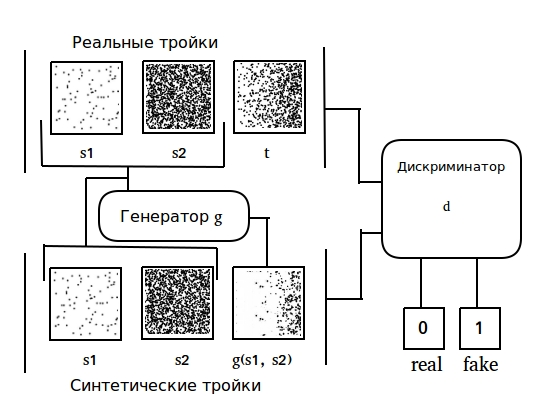
\includegraphics[width=0.65\linewidth]{p2p}}
				\caption{Схематическое устройство сети pix2pix GAN.}
				\label{p2p}
			\end{figure}
			Для pix2pix сети общий функционал потерь выглядит следующим образом: $$ L(G, D) = L_{adv}(G, D) + \eta \mathbb{E}_{p_{data}(s_1, s_2, r)} (\parallel r - G(s_1, s_2) \parallel_1)$$
			$$ L_{adv}(G, D) = \mathbb{E}_{p_{data}(s_1, s_2, r)}\log D(s_1, s_2, r) +  \mathbb{E}_{p_{data}(s_1, s_2)} \log (1 - D(s_1, s_2, G(s_1, s_2)))$$
			где G, D - генератор и дискриминатор, $(s_1, s_2, r)$ - тройка изображений (интенсивность слева, справа и реальное изображение с трендом),  $\mathbb{E}_{p_{data}(s_1, s_2, r)}$ - мат. ожидание логарифмического правдоподобия того, что тройка изображений $(s_1, s_2, r)$ принадлежит вероятностному распределению реальных троек $p_{data}(s_1, s_2, r)$, а $p_{data}(s_1, s_2)$ соответствует распределению реальных изображений $s_1, s_2$.
			\begin{figure}
				\centering{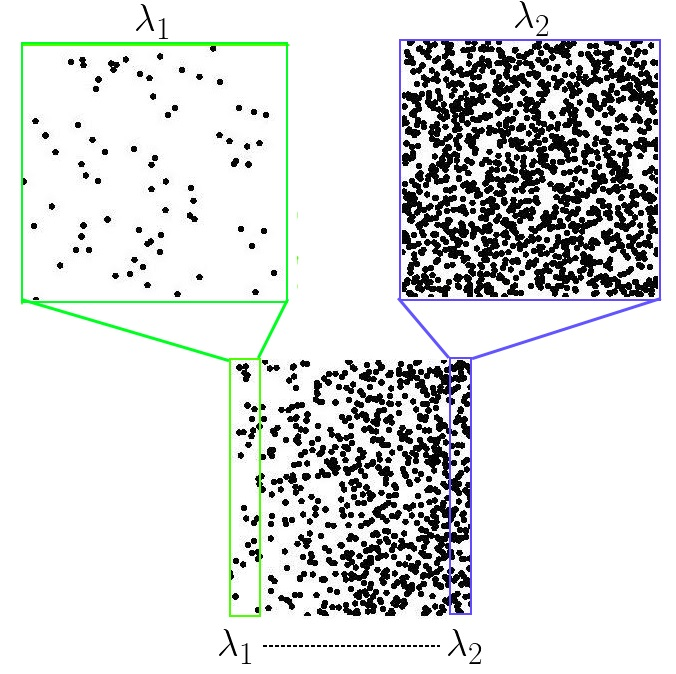
\includegraphics[width=0.75\linewidth]{trend}}
				\caption{Вход и желаемый выход нейросети-генератора.}
				\label{p2p-gen}
			\end{figure}
			\begin{figure}
				\centering{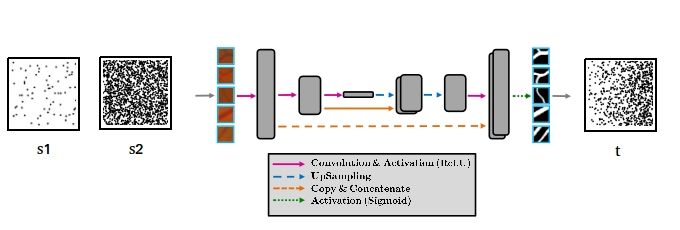
\includegraphics[width=1\linewidth]{unet-scheme}}
				\caption{Схематическое изображение нейросети-генератора.}
				\label{unet-sheme}
			\end{figure}
	% Синтез текстур
	\section{Синтез текстур}
	% Стохастическая оптимизация
	\section{Методы стохастической оптимизации}
	\subsection{Adam}
	\subsection{Nadam}
	% TR-MSE
	\section{Оценка качества синтеза}
	После обучения сети, необходимо проверить, что сгенерированные ей изображения действительно имеют искомые характеристики. Для этого нужно ввести специальную метрику, которая будет учитывать наличие в изображении тренда интенсивности частиц. Было решено использовать среднюю плотность черных пикселей в некотором окне, и проходить этим окном по изображению (Рис. \ref{window}):
	\newpage
	$$\xi_k = \frac{1}{H w}{\sum_{i=k}^{k+w} \sum_{j=0}^{H}\left| \frac{x(i, j) - 255}{255} \right|}, $$$$k = \overline{1, W - w + 1} $$
	\begin{figure}
		\centering{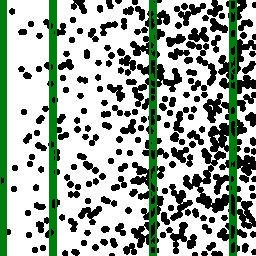
\includegraphics[width=0.35\linewidth]{metrics}}
		\caption{Прохождение окном, W, H - размеры изображения, w - ширина окна.}
		\label{window}
	\end{figure}
	Построив график $\xi(k)$, можно увидеть, как меняется плотность пикселей и прослеживается ли тренд. В качестве метрики можно взять среднеквадратичную ошибку:
	$$ \xi = \frac{1}{W-w}\sum_{k=1}^{W-w+1} (\xi_k - \xi_{0k})^2,$$
	где $\xi_{0k}$ - это $\xi_k$, усредненное по примерам из обучающей выборки. Соответственно, чем меньше значение метрики, тем лучше тренд, присутствующий на сгенерированном изображении, приближает искомый.
	% Результаты
	\section{Результаты}
	Описанные подходы были реализованы в виде компьютерных программ на языке Python с помощью библиотеки для построения искусственных нейронных сетей Keras \cite{keras}, который, в свою очередь, привлекает для расчетов библиотеку Tensorflow \cite{tf}. Обучение проводилось на синтетических данных. 
	\subsection{Выборка с одним трендом}
		Выборка состояла из 6000 обучающих изображений и 316 валидационных. Все изображения содержали в себе различные случайные реализации одного тренда интенсивности
		тут формула
		\subsubsection{GAN}
		\subsubsection{Синтез текстур}
	\subsection{Выборка с множеством трендов}
		\subsubsection{GAN}
		\subsubsection{Синтез текстур}
	\addcontentsline{toc}{section}{ВЫВОДЫ}
	% ВЫВОДЫ
	\section*{\hfil ВЫВОДЫ \hfil}
	Ну вот и чем выводы от результатов отличаются...
	\addcontentsline{toc}{section}{ЗАКЛЮЧЕНИЕ}
	% ЗАКЛЮЧЕНИЕ
	\section*{\hfil ЗАКЛЮЧЕНИЕ \hfil}
	\addcontentsline{toc}{section}{СПИСОК ИСПОЛЬЗОВАННЫХ ИСТОЧНИКОВ}
	\begin{thebibliography}{99}
		\bibitem{Voron-ML}  Воронцов К. В.: "Математические методы обучения по прецедентам (теория обучения машин)".
		\bibitem{CNN-original} LeCun, Y., Boser, B., Denker, J.S., Henderson, D., Howard, R.E., Hubbard, W., Jackel, L.D.: "Backpropagation applied to handwritten zip code recognition" // Neural Comput. 1(4), 541–551, 1989.
		\bibitem{BEGAN} David Berthelot, Thomas Schumm, Luke Metz: "BEGAN: Boundary Equilibrium Generative Adversarial Networks" // arXiv: 1703.10717 [cs.LG], 2017.
		\bibitem{GAN-original} Ian J. Goodfellow, Jean Pouget-Abadie, Mehdi Mirza, Bign Xu, David Warde-Farley, Sherjil Ozair, Aaron Courville, Yoshua Bengio: "Generative Adversarial Nets" // arXiv: 1406.2661 [stat.ML], 2014.
		\bibitem{algorithm-of-articsic-style} Leon A. Gatys, Alexander S. Ecker, Matthias Bethge: "A Neural Algorithm of Artistic Style" // arXiv: 1508.06576 [cs.CV], 2015.
		\bibitem{cGAN-face} Jon Gauthier: "Conditional generative adversarial nets for convolutional face generation", Tech. rep., 2015.
		\bibitem{cGAN} Mehdi Mirza, Simon Osindero: "Conditional Generative Adversarial Nets" // arXiv: 1411.1784 [cs.LG], 2014.
		\bibitem{p2p} Pedro Costa, Adrian Galdran, Maria Inês Meyer, Michael David Abràmoff, Meindert Niemeijer, Ana Maria Mendonça, Aurélio Campilho: "Towards Adversarial Retinal Image Synthesis" // arXiv: 1701.08974 [cs.CV], 2017.
		\bibitem{cond-image-gen-pixelCNN} A\"aron van den Oord, Nal Kalchbrenner, Oriol Vinyals, Lasse Espeholt, Alex Graves, Koray Kavukcuoglu: "Conditional Image Generation with PixelCNN Decoders" // arXiv: 1606.05328 [cs.CV], 2016.
		\bibitem{cond-image-synth-with-clf-GANs} Augustus Odena, Christopher Olah, Jonathon Shlens: "Conditional Image Synthesis with Auxiliary Classifier GANs" // arXiv: 1610.09585 [stat.ML], 2016.
		\bibitem{DC-IGN} Tejas D. Kulkarni, Will Whitney, Pushmeet Kohli, Joshua B. Tenenbaum: "Deep Convolutional Inverse Graphics Network" // arXiv: 1503.03167 [cs.CV], 2015.
		\bibitem{EBGAN} Junbo Zhao, Michael Mathien, Yann LeCun: "Energy-based Generative Adversarial Networks" // arXiv: 1609.03126 [cs.LG], 2016.
		\bibitem{MRF-and-CNN-synthesis} Chuan Li, Michael Wand: "Combining Markov Random Fields and Convolutional Neural Networks for Image Synthesis" // arXiv: 1601.04589 [cs.CV], 2016.
		\bibitem{texture-networks} Dmitry Ulyanov, Vadim Lebedev, Andrea Vedaldi, Victor Lempitsky: "Texture Networks: Feed-forward Synthesis of Textures and Stylized Images" // arXiv: 1603.03417 [cs.CV], 2016.
		\bibitem{texture-synthesis-using-CNN} Leon A. Gatys, Alexander S. Ecker, Matthias Bethge: "Texture Synthesis Using Convolutional Neural Networks" // arXiv: 1505.07376 [cs.CV], 2015.
		\bibitem{keras} François Chollet: Keras, 2015. Software available from http://keras.io/.
		\bibitem{tf} Martín Abadi, Ashish Agarwal, Paul Barham, Eugene Brevdo, Zhifeng Chen, Craig Citro, Greg S. Corrado, Andy Davis, Jeffrey Dean, Matthieu Devin, Sanjay Ghemawat, Ian Goodfellow, Andrew Harp, Geoffrey Irving, Michael Isard, Rafal Jozefowicz, Yangqing Jia, Lukasz Kaiser, Manjunath Kudlur, Josh Levenberg, Dan Mané, Mike Schuster, Rajat Monga, Sherry Moore, Derek Murray, Chris Olah, Jonathon Shlens, Benoit Steiner, Ilya Sutskever, Kunal Talwar, Paul Tucker, Vincent Vanhoucke, Vijay Vasudevan, Fernanda Viégas, Oriol Vinyals, Pete Warden, Martin Wattenberg, Martin Wicke, Yuan Yu, and Xiaoqiang Zheng: "TensorFlow: Large-scale machine learning on heterogeneous systems", 2015. Software available from http://tensorflow.org/.
	\end{thebibliography}
	\addcontentsline{toc}{section}{ПРИЛОЖЕНИЕ}
	\section*{\hfil ПРИЛОЖЕНИЕ \hfil}
	\subsection*{Приложение 1. Использованные версии пакетов}
		\begin{itemize}
			\item Python 3.6
			\item Tensorflow 1.1.0
			\item Keras 2.0.4
		\end{itemize}
	\subsection*{Приложение 2. Еще что-нибудь}
		Еще что-нибудь
\end{document}